\xchapter{Discussão}{}
\label{discussao}


Respostas para perguntas gerais. Fazer uma seção para cada.
Cuidado com a questão das funcionalidades de cada tool -- pode ser o motivo de ser mais usada,
mesmo que não seja sustentável.

\section{Questões} 

Uma questão interessante é a de ``integridade''. 
O que acontece com os resultados anteriores (publicados)
se houver um erro ou uma mudança substancial da forma de calcular algo?
Na prática, só deveríamos permitir refactorings no código 
de um software acadêmico ou adição de novas funcionalidades?
(Chris)

An so what?

O ecossistema de software acadêmico de análise estática sofre de disfunctional ...?

%Encarar o software acadêmico como a "plataforma" do ecossistema de software.
%Pensar no ecossistema de pesquisa e produção intelectual.

Não encontramos relação entre disponibilidade de download e menções, seja Cita, Usa ou Contribui.

\subsection{Q1 - \QuestaoUm}

O software acadêmico tem recebido maior atenção na literatura acadêmica com o
passar do tempo, há uma clara evolução no número total de menções a software
acadêmico de análise estática em publicações das bases ACM e IEEE, conforme
Figura \ref{mentions-by-year}.

\begin{figure}[h]
  \centering
  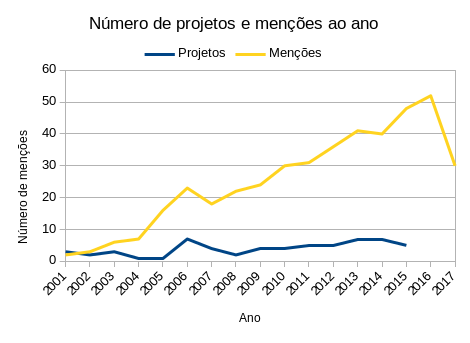
\includegraphics[scale=0.6]{imagens/mentions-projects-by-year.png}
  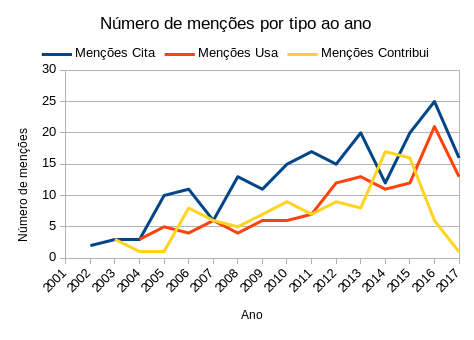
\includegraphics[scale=0.6]{imagens/mentions-type-by-year.png}
  \caption{Número de projetos e menções por tipo ao ano.}
  \label{mentions-by-year}
\end{figure}

Este crescimento, no entanto, é naturalmente influenciado pelo aumento no
número de projetos ao passar dos anos, apesar de ser uma amostra pequena em
números de projetos e terem sido selecionados apenas em publicações das
conferências ASE e SCAM percebe-se um leve crescimento no número de projetos
publicado a cada ano.

%... a Figura \ref{mentions-by-year} (a) é possível notar uma clara relação
%entre o número total de menções e o número de projetos novos por ano, ou seja,
%ao subir o número de projetos sobe também, numa proporção muito maior, o número
%de menções. Quanto mais projetos mais menções, mas também o número de menções
%a software de modo geral cresce ...

%... a Figura \ref{mentions-by-year} (b) apresenta o número de menções por tipo Cita, Usa e Contribui ao
%ano onde é possível notar que ambos os tipos apresentam crescimento similar ao longos dos anos ...

Entretanto, ao analisar o crescimento no número de menções isolando a influência do
crescimento no número de projetos nota-se que a taxa de crescimento isolada do
crescimento de projetos, o número de menções cresce numa taxa de 38\% ao ano,
conforme Figura \ref{mentions-trend}.

\begin{figure}[h]
  \center
  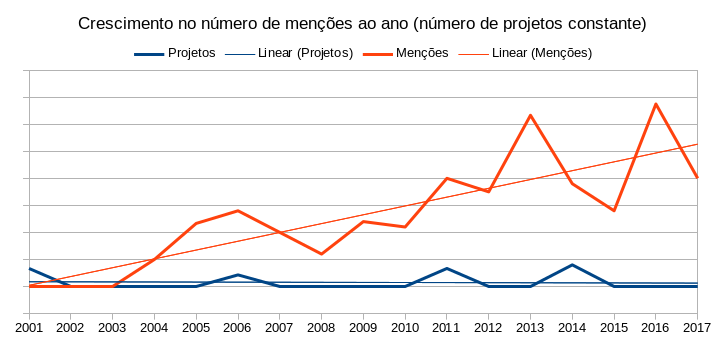
\includegraphics[scale=0.6]{imagens/mentions-trend.png}
  \caption{Crescimento no número de menções por ano (crescimento médio de 38\%).}
  \label{mentions-trend}
\end{figure}

Esta análise para simular um número constante de projetos publicados ao ano foi
realizada selecionando o número de menções ao ano para um conjunto de no máximo
3 projetos selecionados aleatoriamente, visto que o número de projetos em
alguns anos não chega a 3, e para alguns projetos o número de menções é muito
baixa, repetimos esta seleção algumas vezes até obter um número desejável e
calculamos a média do número de menções em cada ano.

%, utilizamos várias amostras de menções por
%ano capturando grupos distintos de no máximo 3 projetos e as menções a estes projetos,
%a taxa de crescimento média de menções ao longo dos anos é de 38\%, ou seja,
%permanecendo constante o número de projetos ao ano, as menções irão crescer numa taxa
%de 38\% ao ano na média ...

\subsection{Q2 - \QuestaoDois} % tamanho médio

O tamanho médio do software acadêmico de análise estática publicado nas
conferências ASE e SCAM é de 820 módulos. Esta média considera a última versão
disponível em código fonte de cada projeto.

%, 22 projetos tiveram seus códigos
%fontes analisados para extrair este dado, os demais projetos não tinham
%código disponível.

O tamanho médio dos projetos em estágio {\it Initial development} é de 595
módulos e são muito menores que os projetos em estágio {\it Evolution} e {\it
Servicing} que é de 1261 módulos na média, os projetos em estágio {\it
Phaseout} e {\it Closedown} não possuem código disponível e portanto não
sabemos o tamanho destes projetos, a Figura \ref{modules-average} apresenta
estes números.

\begin{figure}[h]
  \center
  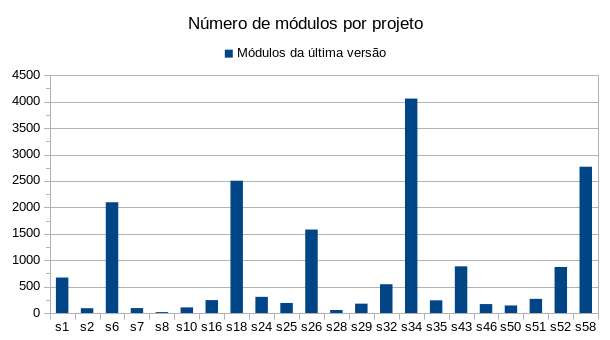
\includegraphics[scale=0.6]{imagens/modules-total.png}
  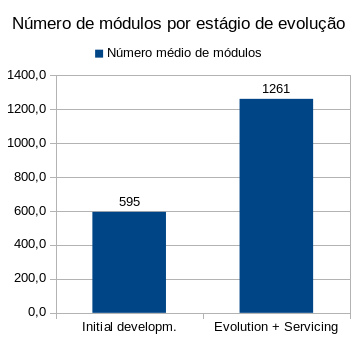
\includegraphics[scale=0.6]{imagens/modules-average.png}
  \caption{Número de módulos por projeto e por estágio de evolução no ciclo de vida.}
  \label{modules-average}
\end{figure}

%(exclui os com valor = 0) são muito menor que osem estágio de evolução e
%serviço  de 1261, ou seja, são pelo menos 2 vezes maior em número de módulos.

São 20 projetos em estágio {\it Initial development}, 12 foram analisados em
código fonte. São 8 projetos em estágio {\it Evolution} e {\it Servicing},
estes dois estágios foram agregados num único conjunto pois possuem
características próximas, e entre os únicos 2 em estágio {\it Evolution} estão
muito mais próximos dos projetos em {\it Servicing} do que {\it Initial
development}. Todos os 8 tiveram código fonte analisado.

%Número médio de módulos

\subsection{Q3 - \QuestaoTres} % idade média

A idade média do software acadêmico de análise estática publicado nas
conferências ASE e SCAM é de 7,6 anos. Foi considerado como ano de nascimento
de cada projeto a data do primeiro lançamento ou da primeira menção ao projeto.
Com isso calculou-se a idade com base no ano de 2017, ou seja, subtraimos 2017
do ano de nascimento.

Ao por em contraste a idade de cada projeto com o número de lançamentos e o
número de menções, conforme Figura \ref{age-releases-mentions}, percebe-se que
a idade dos projetos em {\it Initial development} é superior ao número de
lançamentos, na maior parte é também superior que o número de menções, os
projetos em {\it Evolution} e {\it Servicing} tem natureza contrária, onde o
número de lançamentos é superior a idade, já o número de menções neste estágio
de evolução não é mais disperso.

\begin{figure}[h]
  \centering
  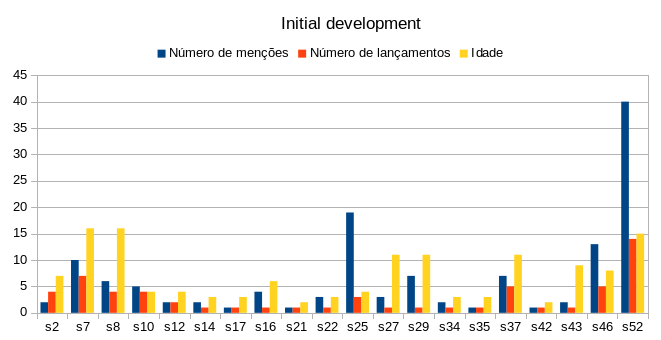
\includegraphics[scale=0.6]{imagens/age-initial-development.png}
  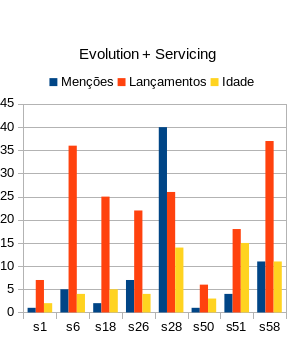
\includegraphics[scale=0.6]{imagens/age-evolution-servicing.png}
  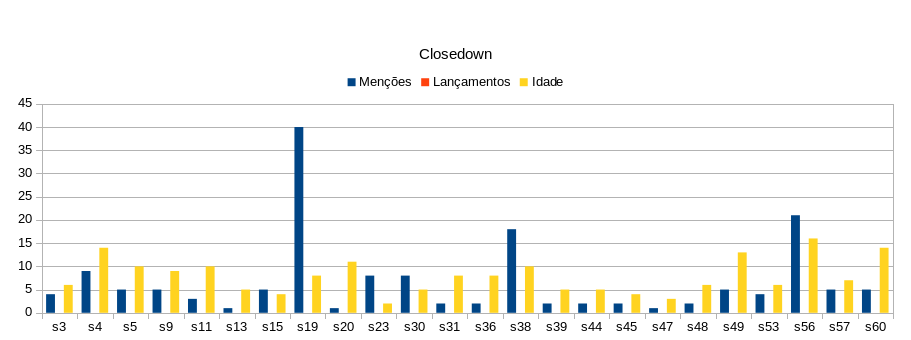
\includegraphics[scale=0.6]{imagens/age-closedown.png}
  \caption{Número de menções, lançamentos e idade de cada projeto por estágio de evoluçao.}
  \label{age-releases-mentions}
\end{figure}

A maior parte dos projetos em {\it Closedown} possuem idade superior ao número
de menções, mas existe excessões, os projetos \texttt{s19}, \texttt{s38} e
\texttt{s56} possui número de menções bem acima da média geral, em especial o
software \texttt{s19} entre os projetos com maior número de menção.
%de menções entre os similar aos dois outros projetos mas que encontram-se em
%initial ou evolution e estão disponiveis para download, inclusive em código
%fonte. Algp que este projeto \texttt{s19} não reflete.


%A idade de cada projeto foi calculada
%considerados todos os anos em que houve lançamento
%ou foram encontradas menções ao software,
%entre todo o período encontrado para cada software, o primeiro ano onde uma
%das ocorrências tenham acontecido, aquela mais antiga, foi considerada como
%Idade VS lançamentos VS menções dos projetos em initial development.
%Idade VS lançamentos VS menções dos projetos em Evolution e Servicing.

%Initial tem idade minima 2 (todos tem essa idade minima ja que a data limite na selecao foi 2015)

A média de idade entre os estágios de evolução é aproximadamente igual, {\it
Evoution} com média 7,3, {\it Initial development} 7,1 e {\it Closedown} 7,9.
A média de idade entre os projetos disponível para download e não disponíveis
para download é o mesmo, 7. Os projetos em estágio {\it Servicing} possuem
entre 4 e 15 anos de idade. A idade mínima de todos os projetos é 2 anos, já
que a revisão de literatura para seleção dos projetos limitou-se ao ano de
2015.

%Mas ao considerar apenas os períodos com lançamentos ou menções, os projetos em
%{\it Evolution} e {\it Servicing} tem média superior
%
%Mas o delta entre a última ocorrencia (release ou mencao) e a primeira é maior,
%nos projetos em servicing e evolution = 7.3,
%enquanto no initial = 4.8 e close = 4.9. Ou seja, se considerarmos a mesma data de nascimento
%mas usar a data final contando a última ocorrência encontrada, seja entre as menções, seja
%entre os lançamentos, os projetos em Servicing e Evolution apresentam um intervalo maior. Isto
%representa que estes projetos tem uma janela de atividade (seja acadêmica, seja fora dela) maior que
%os projetos em Closedown e Initial development.
%
%Importante lembrar que a própria caracterização em relação ao estágio utilizou
%as atividades de lançamento como ponto de partida, não foi o único critério, nem o mais
%definitivo, mas os projetos que tiveram somente uma ocorrência de lançamento ou de menção por exemplo
%foram todos classificados como initial.

%, ou seja, não há entre
%os projetos software mais recente do que 2015.

\subsection{Q4 - \QuestaoQuatro} % reconhecimento

%  13 projetos foram encontrados num único e mesmo artigo já encontrado no estudo anterior
%    (s1, s13, s17, s20, s21, s24, s35, s41, s42, s43, s47, s50, s55)
%  47 foram encontrados em menções
%    17 recebem contribuições
%      (s4, s5, s8, s9, s10, s19, s23, s25, s26, s28, s32, s37, s40, s45, s49, s52, s59)

Entre os projetos em estágio {\it Closedown} foram encontramos 160 menções,
entre os projetos em {\it Evolution} e {\it Servicing} encontrou-se 71 menções,
entre os projetos em {\it Initial development} foi encontrado 131 menções,
a Figura \ref{mentions-stages-total} detalha estes números.

\begin{figure}[h]
  \center
  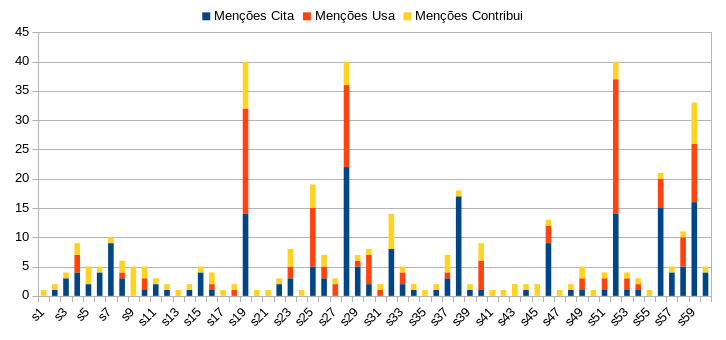
\includegraphics[scale=0.6]{imagens/mentions-by-type.png}
  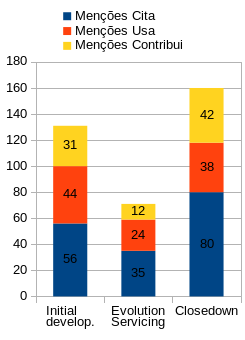
\includegraphics[scale=0.6]{imagens/mentions-stages-total.png}
  \caption{Número total de menções por tipo.}
  \label{mentions-stages-total}
\end{figure}

Não encontramos relação entre o númerp de menções e a característica do projeto
estar disponível para download, mas há uma relação forte entre o uso de
licenças livres e o número de menções, entre 37 projetos sem licença há 200
menções, entre os 23 projetos com licença (38\% menos em comparação com o
número de projetos sem licença) encontrou-se 229 229 menções, ou seja, mesmo
com um número menor de projetos o número de menções encontradas foi 14\% maior.

%... a Figura \ref{mentions-stages-total} ... 

Os projetos \texttt{s19}, \texttt{s38} e \texttt{s56} são os com maior número de
menções entre os projetos em estágio de {\it Closedown}, possuindo menções
recentes entre os anos de 2017, 2016 e 2014, respectivamente.

%      37 sem licença =       200 menções
%-38\% 23 com licença = +14\% 229 menções
%
%      24 sem download =       160 menções
%+50\% 36 com download = +68\% 269 menções
%
%19 projetos acima de 1 menção Contribui
%  260 menções ao total
%  184 lançamentos, 
%  7 closedown, 7 initial, 2 servicing
%
%39 projetos até 1 menção Contribui
%  169 menções
%  119 lançamentos
%  19 closedown, 2 evolution, 13 initial, 1 phaseout, 4 servicing

%1873 (ASE e SCAM) artigos encontrou 60 projetos
%  24 (40\%) não estão disponíveis para download
%  36 (60\%) estão disponíveis para download
%    34 estão disponíveis em código fonte
%      13 não declaram licença
%      21 usam licenças FOSS
%    2 estão disponíveis apenas em binário
%
%busca pelos 60 projetos encontrou 806 artigos (ACM e IEEE)
%  429 menções em 416 artigos
%    199 cita
%    124 usa
%    106 contribui

%Os projedos close possui 38 artigos mencionando uso, estes artigos não são
%possíveis de serem reproduzidos uma vez que possivelmente ter acesso é
%necessário e estes projetos estao sem acesso, 42 artigos contribuindo
%(incluindo o original) também estão fora da possibilidade de serem replicados.

%\begin{figure}[h]
%  \center
%  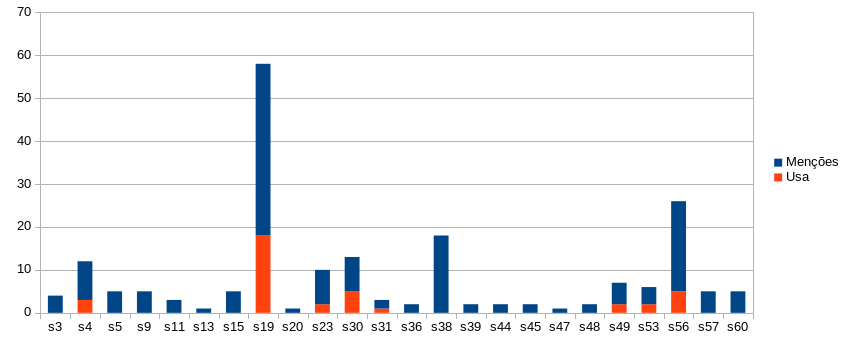
\includegraphics[scale=0.6]{imagens/closedown-mentions-vs-use.png}
%  \caption{Número total de menções em relaçao a menções do tipo {\it Usa} entre os projetos em estágio {\it Closedown}.}
%  \label{closedown-mentions-vs-use}
%\end{figure}

%Média de menções por grupo de estágio de evolução.
%
%\begin{figure}[ht]
%  \begin{minipage}{0.32\textwidth}
%    \centering
%    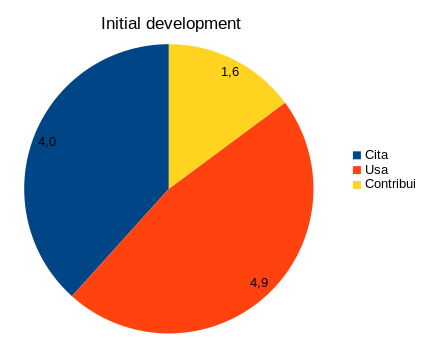
\includegraphics[scale=0.5]{imagens/mentions-initial-development.png}
%  \end{minipage}
%  \begin{minipage}{0.32\textwidth}
%    \centering
%    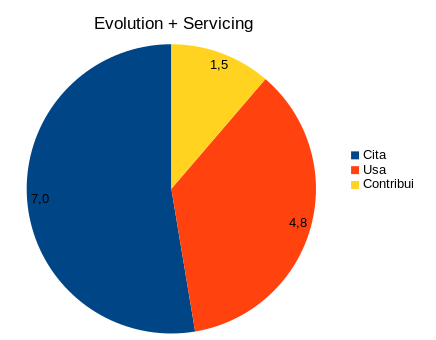
\includegraphics[scale=0.5]{imagens/mentions-evolution-servicing.png}
%  \end{minipage}
%  \begin{minipage}{0.32\textwidth}
%    \centering
%    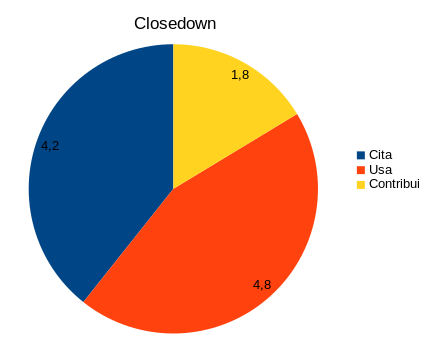
\includegraphics[scale=0.5]{imagens/mentions-closedown.png}
%  \end{minipage}
%  \caption{...}
%  \label{mentions-stages-blah}
%\end{figure}

Entre os projetos em estágio {\it Initial development} apenas 55\% (11) são
livres -- usam licenças de softawre livre --, entre os projetos em {\it
Evolution} e {\it Servicing} a maioria 87\% (7) são livres.

\subsection{Q5 - \QuestaoCinco} % evolução no tamanho

Entre os 60 projetos, 13 não possuem reconhecimento acadêmico, ou seja, são
mencionados no único artigo original publicando o software no ASE ou SCAM pela
primeira vez. Os outros 47 projetos possuem maior reconhecimento acadêmico
(foram encontrados em mais artigos além da primeira publicação). Não há relação
entre as características (número de lançamentos, tamanho em módulos, licença,
disponibilidade de download, etc) do projetos e o reconhecimento acadêmico.

%com reconhecimento
%, entre estes 17 foram
%mencionados em artigos fazendo contribuição, desses 17 10 tem download, 10 tem
%código, 5 initial, 2 servicing, 7 closedown, 3 unknown, 8 tem licença.

Ao analisar a evolução no tamanho em número de módulos dos projetos em estágio
{\it Servicing}, apresentados na Figura \ref{modules-evolution-servicing},
nota-se um crescimento no número total e médio em todos os projetos ao longo
dos anos.

%sem reconhecimento
%), entre
%esses 10 tem download, 9 tem código, 5 initial, 2 evolução, 4 closedown, 1
%phaseout, 1 unknown, 3 tem licença.

\begin{figure}[h]
  \center
  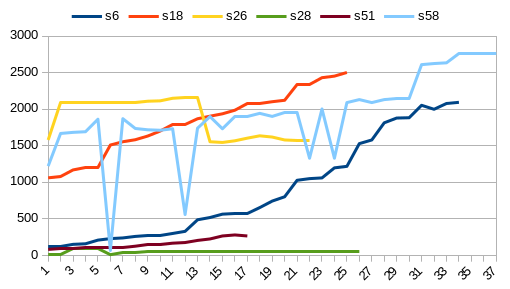
\includegraphics[scale=0.6]{imagens/modules-evolution-servicing.png}
  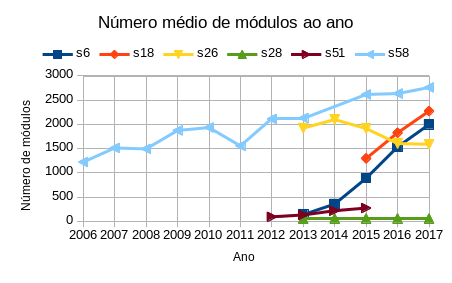
\includegraphics[scale=0.6]{imagens/modules-evolution-average.png}
  \caption{Evolução no número de módulos dos projetos em Servicing.}
  \label{modules-evolution-servicing}
\end{figure}

Ao analisar os projetos individualmente em busca de relação direta entre
menções e o código fonte, encontramos para alguns projetos, mas alguns parecem
ter surgido na academia e seguir totalmente a parte do meio científico, ao
menos entre o que é publicado e indexado nas bases ACM e IEEE.

\begin{description}

  \item[Software \texttt{s6}.]
    Este projeto teve 5 mençoes ao total, em 2015 houve mençao Contribui, em
    2017 apenas menções Cita.
%    ao analisar a evolucao de numero de linhas (eloc) nota-se um pico em 2015.
%    2015 cita e contribui.  2017	cita.

  \item[Software \texttt{s18}.]
    Este projeto foi mencionado em apenas 1 artigo em 2012, sendo que o
    primeiro lançamento da versão 2.0 foi em 2015, este projeto é claramento um
    projeto que ganhou vida própria e segue à parte da academia.

  \item[Software \texttt{s26}.]
    Este projeto foi mencionado em 7 publicações distintas, em 2014 houve
    menção Contribui, nos anos seguintes possui menções de uso e contribuição,
    a princípio é um projeto com ligação estreita com a atividade acadêmica.
    %.  2015	usa.  2016	cita, usa e contribui.

  \item[Software \texttt{s28}.]
    Este projeto está entre os que mais receberam menções, entre 2003 até 2013
    o projeto tem muitas menções, incluindo contribuições, após 2013 apenas
    citações e uso sem mais contribuição após 2013. Possui uma clara ligação
    entre a evolução do projeto e a atividade acadêmica.
%    , o código (modulos e linhas) mostra que até meados de 2014 enfrentou
%    uma grande variação, aparentando um estágio de evolução indicando ser o
%    estado inicial onde faz-se muitas mudanças, após isso entrou em fase de
%    serviço e continua servindo até hoje.

%2003	cita
%2005	cita e usa
%2006	cita e usa
%2007	cita, usa e contribui
%2008	cita e usa
%2009	cita
%2010	cita, usa e contribui
%2011	cita e usa
%2012	cita e usa
%2013	usa e contribui
%2014	cita e usa
%2015	cita
%2016	cita e usa
%2017	cita

  \item[Software \texttt{s51}.]
    Este projeto teve 4 menções ao total e apenas 1 menção Contribui em 2015,
    em 2017 houve menção Cita e Usa. O histórico de lançamentos inicia em 2012
    sendo que as primeiras menções aparecem em 2002, o que nos leva a
    questionar: onde estão os releases anteriores a 2012?

  \item[Software \texttt{s58}.]
    Este projeto foi mencionado 11 vezes, apenas 1 menção Contribui em 2010, as
    demais menções inclui bastante uso do software, entre todos este é o
    projeto com maior janela de tempo entre lançamentos, o histórico de
    lançamentos dá 11 anos. Enquanto a média dos projetos neste estágio de evolução
    é de apenas 4 anos.
  %Evolução do projeto \texttt{s58} em termos de tamanho em número de módulos e número de linhas (eloc).

%2008	menção usa
%2009	menção usa
%2010	contribui
%2011	usa
%2012	cita e usa
%2013	cita
%2016	cita e usa
%2017	cita

\end{description}

%\begin{figure}[h]
%  \centering
%
%  %\begin{minipage}{0.6\textwidth}
%  %  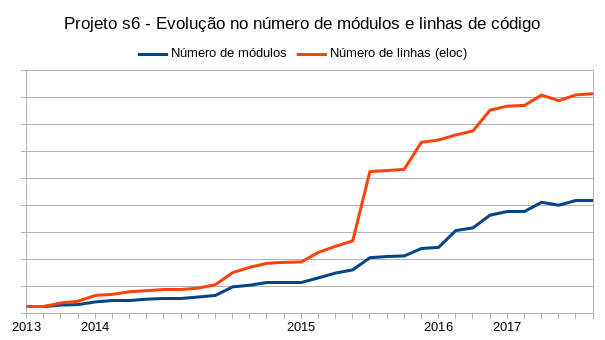
\includegraphics[scale=0.6]{imagens/modules-eloc-s6.png}
%  %\end{minipage}
%  %\begin{minipage}{0.25\textwidth}
%  %  {\small Em 2015 houve mençao contribuindo, poucas menções total, apenas 5
%  %  ao analisar a evolucao de numero de linhas (eloc) nota-se um pico em 2015.
%  %  2015 cita e contribui.  2017	cita.}
%  %\end{minipage}
%
%  %\begin{minipage}{0.6\textwidth}
%  %  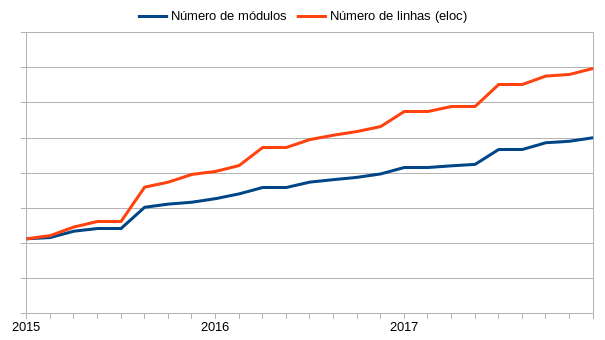
\includegraphics[scale=0.6]{imagens/modules-eloc-s18.png}
%  %\end{minipage}
%  %\begin{minipage}{0.25\textwidth}
%  %  {\small Apenas 1 menção em 2012, primeiro lançamento da versão 2.0 em 2015,
%  %  este projeto é claramento um projeto que ganhou vida própria e segue à
%  %  parte da academia.}
%  %\end{minipage}
%
%  %\begin{minipage}{0.6\textwidth}
%  %  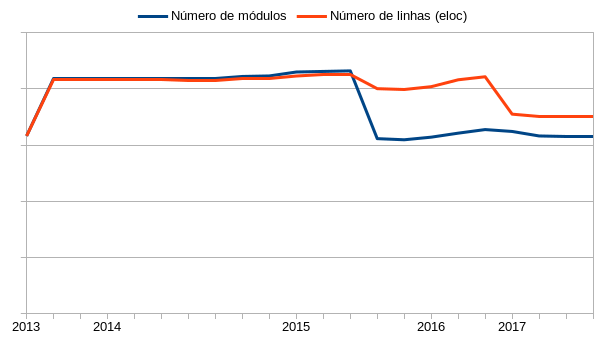
\includegraphics[scale=0.6]{imagens/modules-eloc-s26.png}
%  %\end{minipage}
%  %\begin{minipage}{0.25\textwidth}
%  %  {\small 2014	cita e contribui.  2015	usa.  2016	cita, usa e contribui.}
%  %\end{minipage}
%
%  \caption{Evolução em número de módulos e linhas de código.}
%  \label{modules-eloc-s6}
%\end{figure}

%\begin{figure}[h]
%  \centering
%  \begin{minipage}{0.6\textwidth}
%    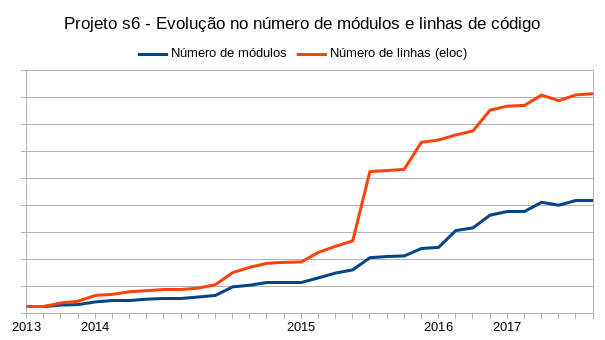
\includegraphics[scale=0.6]{imagens/modules-eloc-s6.png}
%  \end{minipage}
%  \begin{minipage}{0.25\textwidth}
%  {\small Em 2015 houve mençao contribuindo, poucas menções total, apenas 5 ao analisar a
%evolucao de numero de linhas (eloc) nota-se um pico em 2015.  2015	cita e
%contribui.  2017	cita.}
%  \end{minipage}
%  \caption{Evolução do projeto \texttt{s6} em número de módulos e linhas de código.}
%  \label{modules-eloc-s6}
%\end{figure}

%2012	contribui
%  e o histórico de lançamentos
%é após isso, a partir de 2015  (versao 2.0) indicando que as versoes
%anteriores desenvolvido a partir da iniciativa acadêmica não estão publicos
%para efeitos práticos isso n causa problemas mas o historico se perde, onde está o
%código feito ainda na academia, 

%\begin{figure}[h]
%  \centering
%  \begin{minipage}{0.6\textwidth}
%    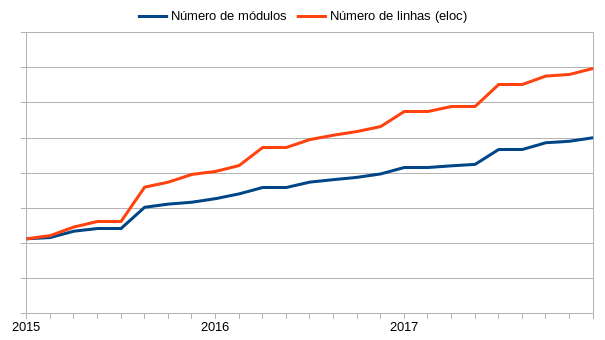
\includegraphics[scale=0.6]{imagens/modules-eloc-s18.png}
%  \end{minipage}
%  \begin{minipage}{0.25\textwidth}
%    {\small Apenas 1 menção em 2012, primeiro lançamento da versão 2.0 em 2015,
%    este projeto é claramento um projeto que ganhou vida própria e segue à
%    parte da academia.}
%  \end{minipage}
%  \caption{Evolução do projeto \texttt{s18} em número de módulos e linhas de código.}
%  \label{modules-eloc-s18}
%\end{figure}

%\begin{figure}[h]
%  \centering
%  \begin{minipage}{0.6\textwidth}
%    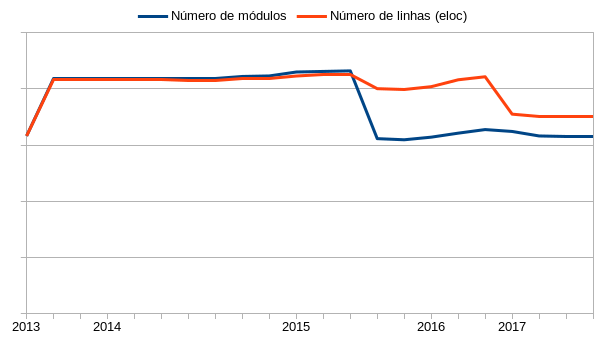
\includegraphics[scale=0.6]{imagens/modules-eloc-s26.png}
%  \end{minipage}
%  \begin{minipage}{0.25\textwidth}
%    {\small 2014	cita e contribui.  2015	usa.  2016	cita, usa e contribui.}
%  \end{minipage}
%  \caption{Evolução do projeto \texttt{s26} em número de módulos e linhas de código.}
%  \label{modules-eloc-s26}
%\end{figure}

%\begin{figure}[h]
%  \centering
%  \begin{minipage}{0.6\textwidth}
%    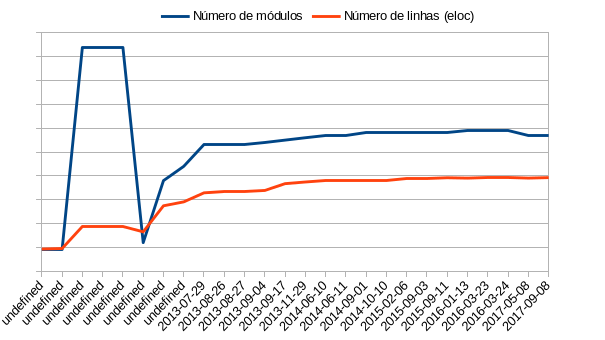
\includegraphics[scale=0.6]{imagens/modules-eloc-s28.png}
%  \end{minipage}
%  \begin{minipage}{0.25\textwidth}
%    {\small De 2003 até 2013 o projeto tem muitas menções, incluindo
%    contribuições, após 2013 apenas citações e uso sem mais contribuição após
%    2013, o código (modulos e linhas) mostra que até meados de 2014 enfrentou
%    uma grande variação, aparentando um estágio de evolução indicando ser o
%    estado inicial onde faz-se muitas mudanças, após isso entrou em fase de
%    serviço e continua servindo até hoje.}
%  \end{minipage}
%  \caption{Evolução do projeto \texttt{s28} em número de módulos e linhas de código.}
%  \label{modules-eloc-s28}
%\end{figure}

%\begin{figure}[h]
%  \centering
%  \begin{minipage}{0.6\textwidth}
%    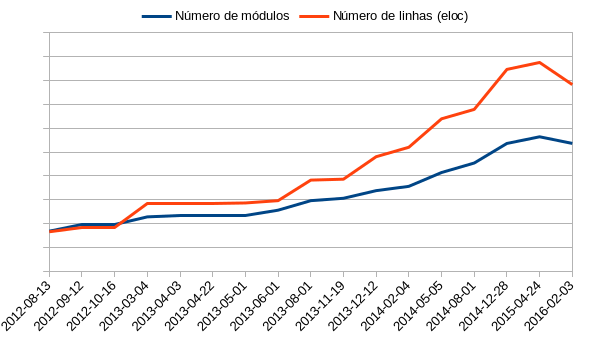
\includegraphics[scale=0.6]{imagens/modules-eloc-s51.png}
%  \end{minipage}
%  \begin{minipage}{0.25\textwidth}
%    {\small o histori de releases conta a partir de 2012 sendo que há enções em
%    2002, onde estao os releases anteriores a 2012? n sabemos.}
%  \end{minipage}
%  \caption{Evolução do projeto \texttt{s51} em número de módulos e linhas de código.}
%  \label{modules-eloc-s51}
%\end{figure}


%\begin{figure}[h]
%  \centering
%  \begin{minipage}{0.6\textwidth}
%    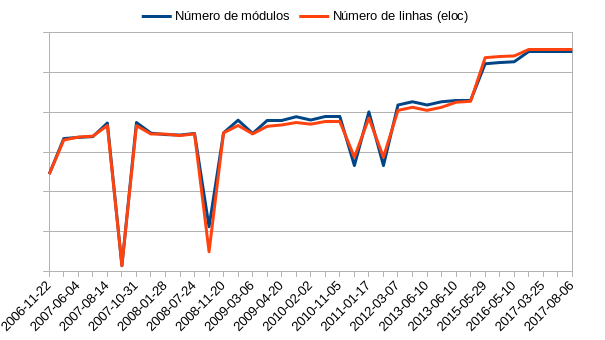
\includegraphics[scale=0.6]{imagens/modules-eloc-s58.png}
%  \end{minipage}
%  \begin{minipage}{0.25\textwidth}
%    {\small Este ...}
%  \end{minipage}
%  \caption{Evolução do projeto \texttt{s58} em termos de tamanho em número de módulos e número de linhas (eloc).}
%  \label{modules-eloc-s58}
%\end{figure}

\subsection{Q6 - \QuestaoSeis} % é útil?

...

\subsection{Q7 - \QuestaoSete} % é sustentável?

...

\section{Trabalhos relacionados}

\citeonline{segal2008developing}
investigam como o desenvolvimento de software acadêmico pode ser melhorado e
enfatiza as diferenças do software acadêmico em relação aos demais tipos de
software, onde o conhecimento sobre o domínio pode muitas vezes incluir temas
avançados e pouco comuns fora do meio científico.

\citeonline{knutson2010report}
ao resumir as conclusões do evento RESER (Workshop on Replication in Empirical
Software Engineering Research) de 2011 cita que ferramentas de software
acadêmico estão indisponíveis ou não são usáveis em estágios não útil, tornando
replicação precisa impraticável.

\citeonline{robles2010replicating} num revisão de 171 artigos do MSR entre 2004 e 2009
em busca de conjunto de dados, artefatos e ferramentas utilizadas nos estudos
necessárias para replicação mostrou que a maioria dos artigos não conseguiram encontrar
as ferramentas mesmo quando o autor explicitamente afirma que fizeram uma.

%\citeonline{holcombe2011openaccess} no projeto {\it Open Access Pledge}
%\footnote{\url{http://www.openaccesspledge.com}} concentra-se em publicar
%softwares e papers em locais de {\it open access}.

\citeonline{portillo2012tools}
através de um mapeamento sistemático mostra que grande parte das ferramentas de
software criadas na academia estão em estado inicial de desenvolvimento que
apenas uma pequena porcentagem são testados fora do contexto onde foi
desenvolvido. 

\citeonline{chaturvedi2013tools}
faz uma revisão de literatura entre artigos submetidos ao MSR de 2007 até 2013,
identifica conjunto de dados, ferramentas e técnicas utilizadas pelos autores,
mais da metade dos artigos usam ou criam ferramentas, categoriza as ferramentas
em ferramentas novas, ferramentas tradicionais, protótipos e scripts para
mineração de dados.

\citeonline{barnes2013science}
cria o manifesto {\it Science Code Manifesto} e enfatiza que todo código fonte
escrito especificamente para processar dados de publicações devem estar
disponíveis aos revisores e leitores do paper.

\citeonline{marshall2013tools} num mapeamento sistemático sobre artigos criando
ferramentas de apoio a revisão sistemática no domínio de SE conclui que as
ferramentas encontradas estão em estado inicial de desenvolvimento.

\citeonline{hettrick2014uk} mostra que no reino unido entre todas as áreas da
ciência 56\% dos cientistas estão envolvidos no desenvolvimento de software
acadêmico.

\citeonline{wilson2014best} resume as melhores práticas para melhoria da
manutenibilidade e disponibilidade do software acadêmico desenvolvido por
cientistas.

\citeonline{wilson2014software} num resumo sobre as lições aprendidas em 20
anos da iniciativa {\it Software Carpentry} sobre atividades de melhoria das
habilidades dos pesquisadores com computacao.

\citeonline{amann2015software}
investigam através de uma revisão sistemática de literatura uma década de
publicações e encontram que muito poucos estudos são replicáveis visto que
faltam informações incluindo dados e ferramentas, apenas 20\% dos estudos
possuem ferramentas disponíveis.

\citeonline{momcheva2015software}
num survey com 1142 participantes sobre o uso de software em pesquisas da
astronomia mostrou que 90\% dos cientistas escrevem software e 100\% usam
software em suas pesquisas.

\citeonline{beller2016analyzing} avalia e sugere caminhos para melhorar o
desenvolvimento de ferramentas de análise estática com o objetivo de aumentar a
adoção.

\citeonline{smith2016software} resume recomendações sobre como citar software
na literatura acadêmica com objetivo de encorajar uma ampla adoção e uma
política consistente para citação de software entre as múltiplas disciplinas.

\citeonline{smith2016software} afirma que ``citações aos softwares devem
permitir e facilitar acesso ao software, metadados, documentação, dados e
outros materiais necessários tanto para humanos quanto para máquinas''.

%\citeonline{wilkinson2016fair} através do {\it FAIR
%principles}\footnote{\url{https://www.nature.com/articles/sdata201618}} com
%foco em dados de pesquisa, o objetivo é fazer eles serem encontráveis,
%acessíveis, interoperável e reusável. Estes princípios podem ser generalizados
%para aplicar aos softwares.

\citeonline{howison2016software}
numa revisão de literatura mostrou que publicações usando softwares como
método, mostrou que apenas 59 mencionavam o uso de softwares de alguma forma,
os demais 31 artigos, apesar de usar software acadêmico, não mencionavam nada a
respeito.

\citeonline{wilson2017good} apresenta um conjunto de boas práticas que todo
pesquisador pode adotar, independentemente do seu nível de habilidade em
computação. Essas práticas passam por gerenciamento de dados, programação,
colaboração com colegas, organização de projetos, tracking work, e escrita da
manuscritos.
%, sao desenhados para uma grande variadade de fontes publicadas do
%noso dia a dia e do nosso trabalho como voluntário organizando workshopts desde
%2010.

%Open Science Peer Review Oath\footnote{\url{https://f1000research.com/articles/3-271/v2}}
%Concentra-se em potencializar os revisores para exigir acesso aberto aos
%softwares, práticas reprodutíveis e revisões transparentes.

%Muitos pesquisadores não
%disponibilizam os seus softwares 
 %ou quanto o fazem enfrentam problemas com disponibilidade e
%manutenibilidade \cite{prlic2012ten}
